\documentclass{article}%
\usepackage[T1]{fontenc}%
\usepackage[utf8]{inputenc}%
\usepackage{lmodern}%
\usepackage{textcomp}%
\usepackage{lastpage}%
\usepackage[head=40pt,margin=0.5in,bottom=0.6in]{geometry}%
\usepackage{graphicx}%
%
\title{\textbf{Mueren cuatro jóvenes tras procedimiento policial en Filas de Mariche}}%
\author{Diario El Universal}%
\date{24/09/2018}%
%
\begin{document}%
\normalsize%
\maketitle%
\textbf{URL: }%
http://www.eluniversal.com/sucesos/21378/mueren{-}cuatro{-}jovenes{-}tras{-}procedimiento{-}policial{-}en{-}filas{-}de{-}mariche\newline%
%
\textbf{Periodico: }%
EU, %
ID: %
21378, %
Seccion: %
sucesos\newline%
%
\textbf{Palabras Claves: }%
NO\_TIENE\newline%
%
\textbf{Derecho: }%
1.1%
, Otros Derechos: %
NO\_TIENE%
, Sub Derechos: %
1.1.1.9%
\newline%
%
\textbf{EP: }%
NO\newline%
\newline%
%
\textbf{\textit{Las víctimas fueron heridas por arma de fuego y luego fueron traslados a un Centro de Diagnóstico Integral cercano a la zona, donde fallecieron según dijeron familiares.}}%
\newline%
\newline%
%
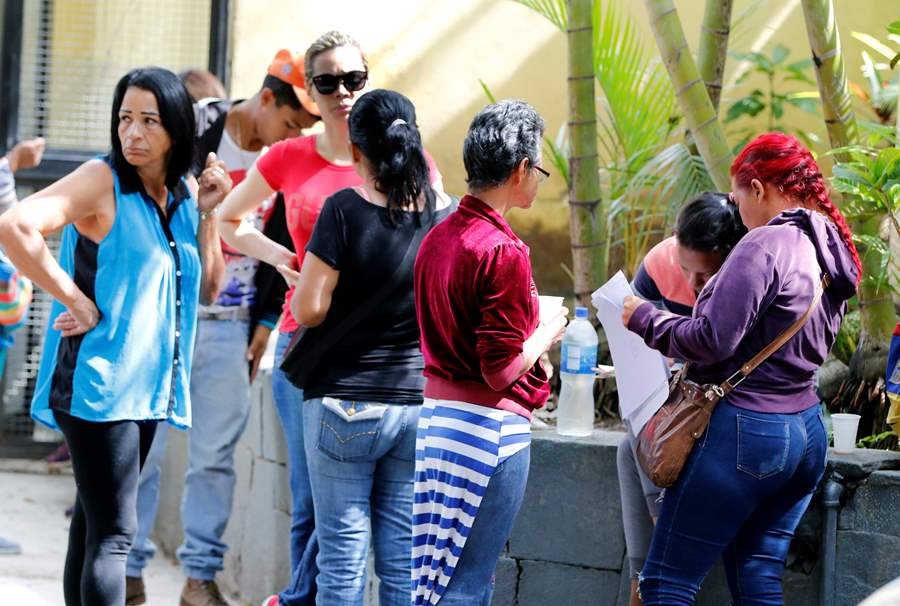
\includegraphics[width=300px]{258.jpg}%
\newline%
%
Caracas.{-}~Alrededor de las 4:00 de la mañana del viernes, una comisión policial realizó un procedimiento en diferentes residencias en el sector Villa Tatiana, Filas de Mariche, municipio Sucre, donde murieron cuatro personas.%
\newline%
%
Hasta el momento, los fallecidos identificados son Gregori Moisés Coronado León, de 26 años; Adrián Jesús Sanabria, de 23 años, y Gari Prieto Corrales, de 28.%
\newline%
%
Este domingo, sus familiares se acercaron a la morgue de Bello Monte para conocer las circunstancias de los decesos y retirar los cuerpos.%
\newline%
%
Según la versión de los allegados, las víctimas fueron heridas por arma de fuego y luego fueron traslados a un CDI cercano a la zona, donde fallecieron.%
\newline%
%
Familiares de Coronado León aseguraron que la víctima era taxista de la Asociación Civil Unión de Conductores Bolivarianos de La Lagunita y dejó un hijo.%
\newline%
%
Por otra parte Nelly Martínez, abuela de Sanabria, expresó que cuando llegaron los funcionarios "Adrián estaba durmiendo en su casa". Dice que "si una persona cometió un delito y los agarran sin armas, sin disparar, llévatelo preso y entrégalo a la justicia". Sobre el hecho  dijo que "tiene que haber una averiguación a fondo". \newline%
Mencionó que Sanabria no estuvo detenido anteriormente, trabajó en una panadería en  la zona donde residía y dejó dos hijos.%
\newline%
%
\end{document}